\documentclass[10pt,twocolumn,letterpaper]{article}

\usepackage{cvpr}
\usepackage{times}
\usepackage{epsfig}
\usepackage{graphicx}
\usepackage{amsmath}
\usepackage{amssymb}
\usepackage{color}

% Plotting fun :D
\usepackage{tikz,pgfplots}

\newcommand{\preliminary}[1]{\textcolor{red}{#1}}

\usepackage{color}
\newcommand{\todo}{\colorbox{yellow}{\fbox{\LARGE{TODO}}}}

% Include other packages here, before hyperref.

% If you comment hyperref and then uncomment it, you should delete
% egpaper.aux before re-running latex.  (Or just hit 'q' on the first latex
% run, let it finish, and you should be clear).
\usepackage[pagebackref=true,breaklinks=true,letterpaper=true,colorlinks,bookmarks=false]{hyperref}

% \cvprfinalcopy % *** Uncomment this line for the final submission

\def\cvprPaperID{****} % *** Enter the CVPR Paper ID here
\def\httilde{\mbox{\tt\raisebox{-.5ex}{\symbol{126}}}}

% Pages are numbered in submission mode, and unnumbered in camera-ready
\ifcvprfinal\pagestyle{empty}\fi
\begin{document}

%%%%%%%%% TITLE
\title{What If Localization Worked?}

\author{First Author\\
Institution1\\
Institution1 address\\
{\tt\small firstauthor@i1.org}
% For a paper whose authors are all at the same institution,
% omit the following lines up until the closing ``}''.
% Additional authors and addresses can be added with ``\and'',
% just like the second author.
% To save space, use either the email address or home page, not both
\and
Second Author\\
Institution2\\
First line of institution2 address\\
{\tt\small secondauthor@i2.org}
}

\maketitle
%\thispagestyle{empty}

%%%%%%%%% ABSTRACT
\begin{abstract}
   Real world computer vision systems typically have some intrinsic value in their underlying business use. Serving the the right image in a search result ad might be worth \$0.001 and counting nuclear particles in material images might be worth \$10,000. In general, we want to build systems which produce sufficiently accurate results within a given budget. Although an interaction with human workers can improve accuracy in many algorithms, it also increases the cost. Most computer vision research focuses on purely automated algorithms, arguing that human labor is much too expensive to be included as subroutines in operational algorithms. In this work, we put this argument into perspective by investigating joint algorithms using computers and human labor. In particular, we focus on how different degrees of human involvement effect the algorithm's accuracies. We focus on the representative computer vision task of localization, however, our general methodology can similarly be applied to other tasks, e.g., Object Detection or Image Matching. We introduce several general strategies for combining existing computer vision algorithms with human labor, e.g. (To be filled). We evaluate our results on three reference data sets, i.e., UIUC Cars, Caltech Pedestrian and Street View House numbers, and show how the accuracy of the algorithms scale with varying degrees of human involvement. Finally, we provide an outlook on what computer vision applications become possible, if localization works.
\end{abstract}

%%%%%%%%% BODY TEXT
\section{Introduction}

\section{Localization}
\preliminary{
A place to describe
\begin{enumerate}
\item definition of what we understand it is
\item Where localization fits into a typical classification pipeline, which helps us motivate why we chose to focus on this problem in particular
\item state of the art
\item data sets
\item applications
\end{enumerate}
}

% Contributed by students:
\preliminary {
Object localization is one of the most obvious parts of any computer vision application. It involves two basic tasks namely semantic segmentation and object detection. Semantic segmentation is the task of labelling the pixels of an image depending on their semantic category while object detection produces a rough location (bounding boxes) of all the instances that belong to a set of objects of interest. Our research focuses more on object detection. Object detection allows us to count the number of objects precisely, which is not always possible from semantic segmentation.
Where does localization fit into a typical classification pipeline? This helps us motivate why we chose to focus on the problem of localization in particular( to be done)
These are some previously proposed papers on object localization using different techniques~\cite{localization01,localization02}. Although these papers provide various impressive techniques, we through our paper would like to improve upon the accuracy of the localization algorithm by incorporating HPU component with it.
}

\preliminary{
\todo We're going to have to be extremely consistent with how we use our terminology. ``Detection''? ``Localization''? What's the difference? After we decide this (and this section is probably a good place to choose), we should do a Ctrl+F on all instances of both words and change them to match.
}


\section{Data Sets}
\preliminary{
\begin{enumerate}
\item in detail the picked data sets (refer to previous section why they are important.)
\item the measure of accuracy on those data sets
\end{enumerate}
}

\subsection{UIUC Cars}\label{sec:uiuc-cars}
For our first example, we chose the classic UIUC cars dataset, introduced in~\cite{agarwal2002learning,agarwal2004learning}. This dataset makes a particularly good baseline because it is well-established and because there is no recognition task after the initial detection/localization step. This dataset allows us to measure the performance of a simple single-class open-set detection task. The 550 positive samples in the test set are side views of cars, some of which are partially occluded, and the 500 negative training samples contain natural scenes, various other vehicles, etc.

On this dataset, performance is evaluated using standard precision/recall measures. F-measure and absolute number of false positives is also typically reported. In the single-scale case, the output bounding box is 100$\times$40px, and it counts as a correct detection if the center lies within a certain ellipse of the groundtruth's bounding box center. Since there may be many cars per image; statistics are aggregated over each individual car in the test set, not per image. The original parts-based representation in~\cite{agarwal2002learning} achieves about 77.58\% F-measure.

\preliminary{\todo What is the state of the art?}


\subsection{Caltech Pedestrian Detection Benchmark}
The Caltech Pedestrian Detection Benchmark, introduced by~\cite{dollarCVPR09peds}, is a challenging pedestrian detection dataset. This set is several orders of magnitude larger than the UIUC~Cars set, containing 350,000 groundtruth pedestrian bounding boxes. The research that uses this dataset is summarized by~\cite{Dollar2012PAMI}.

To evaluate performance, this dataset asks authors to calculate a standard ROC curve of their detection results. However, in the open set ``self-driving car looking for pedestrians'' scenario, the amount of negative data is potentially infinite, which means plotting TP/TR is not very insightful. Instead, authors report miss rate versus number of false positives per image (``\emph{FPPI}''). This ROC curve is summarized as the ``\emph{log-average miss rate,}'' computed by averaging the miss rate at nine FPPI values along logarithmically-spaced intervals~\cite{Dollar2012PAMI}.

A detection counts as correct if its intersection-over-union score is greater than 0.5, meaning $\frac{\textsc{Area}(A \cap B)}{\textsc{Area}(A \cup B)} \geq 0.5$, where $A$ and $B$ are the detected and groundtruth bounding boxes respectively.

\subsection{Street View House numbers}
\cite{netzer2011reading}

\preliminary{Problem: The first paper that uses this dataset \cite{netzer2011reading} only reports classification accuracy, which is separate from the precision/recall tasks. It's unclear to me where they're assuming they have groundtruth segmentation and where they do not start from the crop set. We might be able to spin the story as ``Well what if it wasn't already solved? How would the existing algorithms perform if they didn't already have good crops? And how can we minimize this performance drop? This is a hard problem and nobody's thinking about it''. Or we could just pick a different dataset. Not sure.}

\preliminary{Question for you guys: did anyone find previous work that measures localization accuracy on this dataset?}

\section{Computer-Human Localization}
\preliminary{
A place to describe
\begin{enumerate}
\item Our different HCOMP algorithms
\item Examples
\item Evaluations (the famous plots we always talk about)
\end{enumerate}
}


% Contributed by Team BlackHatProcrastinators
% \preliminary{
% The presented algorithm is a real time implementation of HPU. In this the window is to be divided into two parts i.e. first part is to surf for the images of the car and the second part is to drag and drop the respective image. CPU algorithm is detecting the points of the parts of the objects like wheels, car window etc.If the detected parts are correct then one can go onto the next image and if not then by placing the points on it’s correct part.
% The user would be given a threshold time of 9 sec for each image once they have dragged and dropped the image to make any changes. Once the threshold time is reached the drag and drop part of the window will itself clear the image and once again the user can drag the image.


% HPU Algorithm
% This algorithm has been designed for the UIUC dataset, but can work with any dataset in general. We have created 3 versions of our algorithm so far. The algorithm given below is the 3rd version out of all that we created. The other 2 versions, their design process and philosophy may be found in our assignment submission for this week.

% In our algorithm we take 2 strategies to exploit the differences of the real world:
% Latency factor of Humans (as an indicator for image complexity)
% Skill level of Humans (for optimal distribution of images)

% Every person takes different amount of time to process different types of images. A simple image will take less time and a complex image will consume more time.

% In our algorithm we take an image to be “complex” if it satisfies one or more of the following:
% All the desired objects can’t be identified properly.
% The image takes relatively more computation time.

% We take “performance” as a measure inversely proportional to the time taken by a user.
% We store just a boolean variable of “smartness” against every user based on their latest performance.


% Assumptions:
% A complex image is more prone to errors than a simple image.
% Hence based on the complexity of images we shall dynamically vary the number of reviewers for any image.
% For now let us assume that, images demanding relatively more CPU time, are challenging for humans as well (i.e, it is a complex image). This assumption can be relaxed as soon as we find a proper correlation between the particular CV algorithm (that we are using) and the complexity posed to human classifiers.

% Ultimately we want the CPU to identify which image should be given to a “smart user” and which image can be handled, even by “not so smart users”.
% This would result in the minimum time requirement, and an optimal utilization of human resources.

% HPU_Version3 :
% Each image along with the probable bounding boxes (found by the CV algorithms) will be shown to:
% 3 “smart” people if image is complex, set Time_Threshold = 7sec
% 3 “not so smart” people for simple images, set Time_Threshold = 10sec
% 		Start recording the time for every user
% If all the cars are identified correctly:
%     i.         Press Yes
%        b.   If all the cars are NOT identified correctly:
%      i.        Select ones which are perfect
%     ii.        Rescale imperfect boxes
%    iii.        Add new boxes which were missed.
% (Based on the Person who marks the box a unique edge colour will be given to the bounding box)
%         2.  If Avg_Time_Spent < Time_Threshold, then show  these images to a set of 5 people.
% Else, if the Avg_Time_Spent >= Time_Threshold, then the images will be shown to a set
% of 7 people. They will have to do the following :
% If there is at least one correct bounding box around every car:
% Select one bounding box for each car image
%        b. Else:
%                                    ii.    Click “Report this Image”
%       3.  Based on which bounding box was chosen by the maximum people, that particular
%             box will be marked as the final bounding box for that image.
%       4.  If there is an image whose majority voting says “Image Reported Wrong”, it will be
%             resent for processing.



% Cost
% We propose to take time as a unit to measure cost. We will also attach different weights to different actions (performed by the user), such as Clicking Yes/No, Resizing Bounding boxes, Creating new Bounding boxes etc.

% Using statistical analysis, we can find out the closest ideal time for a particular task. eg. Median of the times might be one good measure.

% Weights can be assigned as a function of the different tasks performed :
% W1 (lowest weight) - Clicking Yes/No for the correctness of bounding boxes
% W2  (medium weight) - Resizing bounding boxes for better accuracy
% W3  (highest weight) - Creating new bounding boxes in place of the old ones

% This would take into account the complexity factor for any type of task.

% Therefore, Cost = Weight of a given task * Time taken by user to do the task


% HPU Integration:
% We present a novel approach for HPU integration in this project. The Human skill and intelligence to find objects in cluttered environment could be used as a feedback for the trained localization algorithm. Eg. a trained localizer will predict the object location in an image. Then the same image will be presented before HPU for marking ROI. Percentage overlap will be calculated and the data will be feed back the to algorithm. Just as BackPropagation algorithm works in a Neural Network, we propose this feedback method to improve the accuracy of the localizer.
% Cost:
% Cost will be calculated as the time required by the HPU to mark the bounding box around the ROI in the image.

% Cost-effective HPU
% The HPU we have implemented aims on reducing the number of tasks sent out to the human workers. Instead of passing an image large number of times to converge to a highly-likely label, we pass the image individually lesser number of times to get an initial guess. Once, an initial guess is obtained we cluster similarly marked images and send a cluster to a worker (in a single HPU task). All that the worker needs to do is mark the one which is falsely classified thus also implicitly verifying correctness of others in the cluster.

% For example, in case of the UIUC data set the HPU can find the odd one out by checking if there is an empty/non-car bounding box. This can have couple of advantages over other HPU methods being implemented. With few initial passes of asking worker to draw correct bounding boxes we can ensure that we get the marking for the false negatives. Subsequent passes can be made via our proposed approach. This will help in pruning false positives and confirming true positives in a single pass. Thus, reducing number of HPU tasks.
% }


\subsection{UIUC Cars}
\begin{figure}[t]
  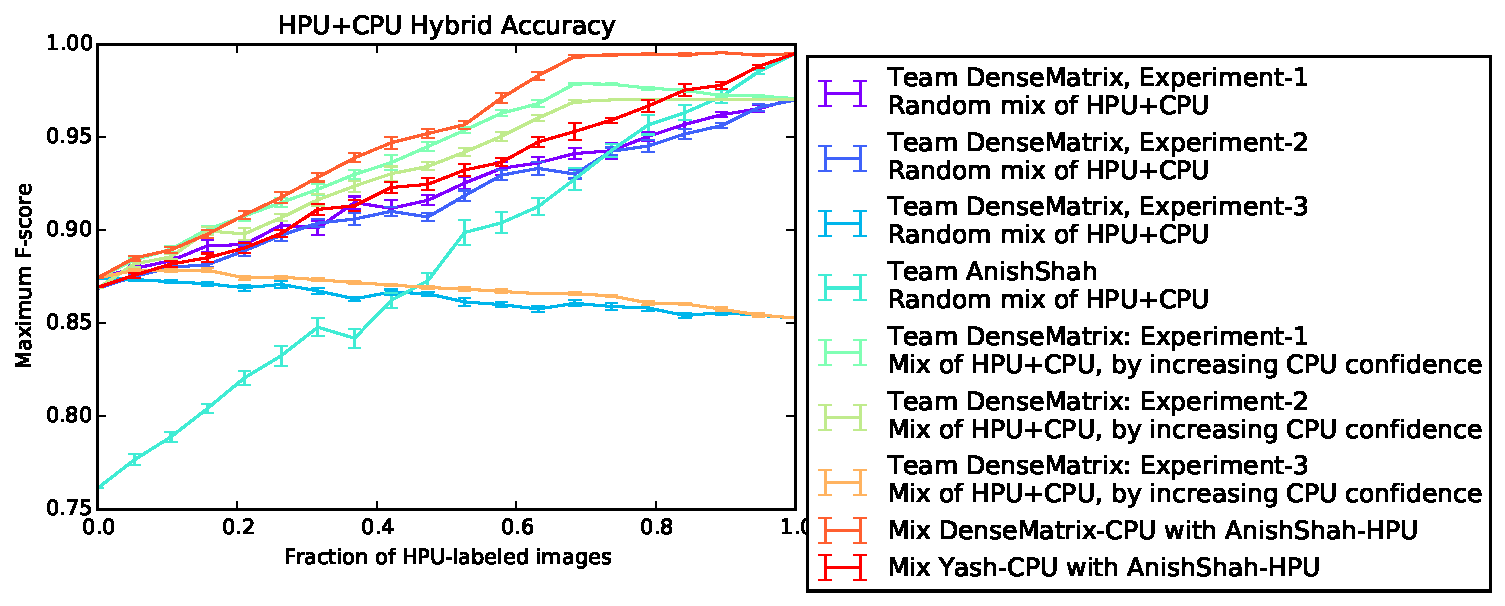
\includegraphics[width=1\linewidth]{figure-UIUC-Cars-acc-vs-fraction.pdf}
\end{figure}

\todo Team DenseMatrix: What is the difference between HPU Experiments 1, 2, 3? Please describe exactly what the task was, whether you started from CPU or HPU bounding boxes, etc.

\todo Team AnishShah, Yash's team: Please include confidence values for each bounding box in your CPU results. That way, we can ask the human worker to label the least-confident images first, which will help quickly improve performance

\todo Team DenseMatrix: Thanks for including confidence values, but they are taken from the set $\{1, 2\}$. Is there any way to get confidence more fine-grained?

\subsection{Caltech Pedestrians}
\begin{figure}[t]
  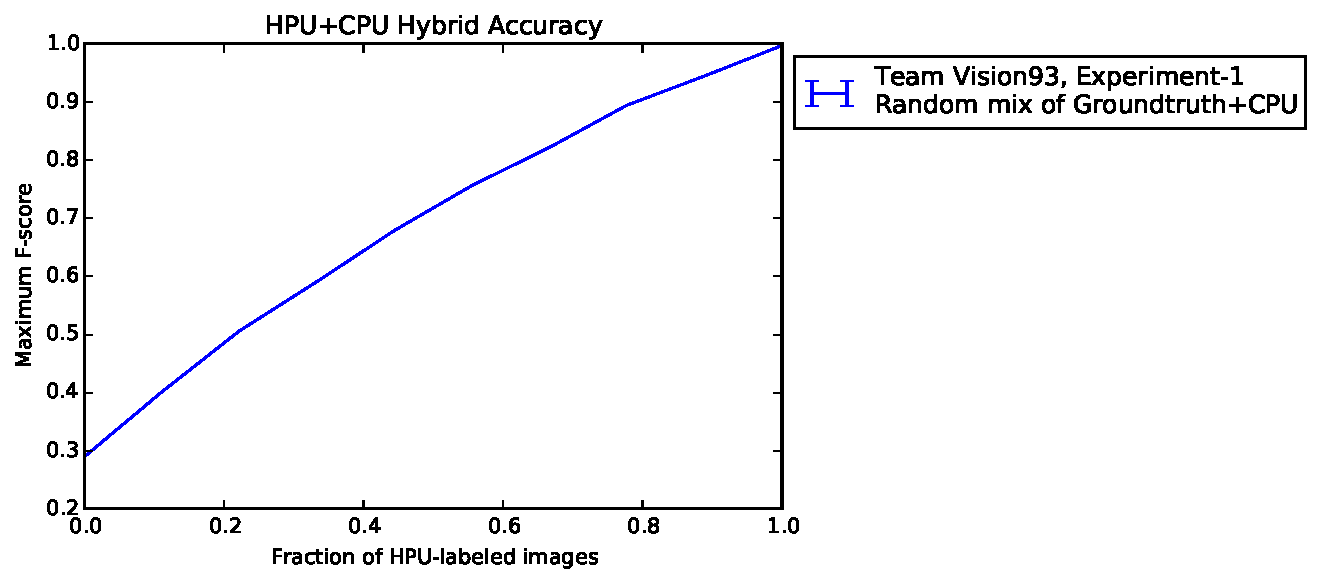
\includegraphics[width=1\linewidth]{figure-Pedestrians-acc-vs-fraction.pdf}
\end{figure}

\todo Team Vision93: Thanks for including bounding boxes, but we note that the groundtruth has 4,024 images and your CPU results list bounding boxes for 1,400 images. Is this intentional? This would mean that the CPU algorithm starts at $\approx$ 30\% recall.

\todo All teams: Does anyone have bounding boxes for Caltech?


\subsection{Street view house numbers}
\todo All teams: It looks like we may have to come up with our own strategy to evaluate SVHN.


\section{Applications}
\preliminary{
A place to describe
\begin{enumerate}
\item Now that we've shown that we can improve accuracy, what other applications can we enable?
\item Graph that shows, human labour cost vs, profit of company/test... (the graph is generated by intersecting(or whatever maximization is needed between cost/accuracy and value/accuracy)
\end{enumerate}
}

\section{Conclusion}

%-------------------------------------------------------------------------


{\small
\bibliographystyle{ieee}
\bibliography{egbib}
}

\end{document}
